\documentclass[11pt,a4paper]{article}

% -----------------------------------------------------------------------------
% Language and typography
% -----------------------------------------------------------------------------
\usepackage[T1]{fontenc}
\usepackage[utf8]{inputenc}
\usepackage[english]{babel}
\usepackage{lmodern}
\usepackage{microtype}

% -----------------------------------------------------------------------------
% Page layout
% -----------------------------------------------------------------------------
\usepackage[
    top=2.5cm,
    bottom=2.5cm,
    left=2.7cm,
    right=2.7cm,
    headheight=15pt
]{geometry}

\setlength{\parindent}{1.25cm}
\setlength{\parskip}{0.25em}
\setlength{\emergencystretch}{2em}

% -----------------------------------------------------------------------------
% Graphics, colors and boxes
% -----------------------------------------------------------------------------
\usepackage{graphicx}
\usepackage{xcolor}
\usepackage[most]{tcolorbox}
\usepackage{caption}

\definecolor{documentblue}{HTML}{17365D}
\definecolor{lightblue}{HTML}{F3F7FB}
\definecolor{mediumgray}{HTML}{666666}

\captionsetup{
    font=small,
    labelfont=bf,
    justification=centering
}

% -----------------------------------------------------------------------------
% Lists and section headings
% -----------------------------------------------------------------------------
\usepackage{enumitem}
\usepackage{titlesec}

\setlist[itemize]{
    leftmargin=1.8em,
    itemsep=0.25em,
    topsep=0.4em
}

\setlist[enumerate]{
    leftmargin=1.8em,
    itemsep=0.25em,
    topsep=0.4em
}

\titleformat{\section}
    {\Large\bfseries\color{documentblue}}
    {\thesection}
    {0.75em}
    {}

\titleformat{\subsection}
    {\large\bfseries\color{documentblue}}
    {\thesubsection}
    {0.75em}
    {}

\titleformat{\subsubsection}
    {\normalsize\bfseries}
    {\thesubsubsection}
    {0.75em}
    {}

\titlespacing*{\section}{0pt}{2.2em}{0.8em}
\titlespacing*{\subsection}{0pt}{1.7em}{0.6em}
\titlespacing*{\subsubsection}{0pt}{1.3em}{0.4em}

% -----------------------------------------------------------------------------
% Headers and footers
% -----------------------------------------------------------------------------
\usepackage{fancyhdr}

\pagestyle{fancy}
\fancyhf{}

\fancyhead[L]{\small EASN-FW}
\fancyhead[R]{\small Software Requirements Specification}
\fancyfoot[C]{\small \thepage}

\renewcommand{\headrulewidth}{0.4pt}
\renewcommand{\footrulewidth}{0pt}

% -----------------------------------------------------------------------------
% Hyperlinks
% -----------------------------------------------------------------------------
\usepackage[
    colorlinks=true,
    linkcolor=documentblue,
    urlcolor=documentblue,
    citecolor=documentblue,
    pdftitle={Software Requirements Specification for Ecoacoustic Sensing Node},
    pdfauthor={Henrique Sander Lourenço, João Colombari}
]{hyperref}

% -----------------------------------------------------------------------------
% Tables
% -----------------------------------------------------------------------------
\usepackage{array}

% -----------------------------------------------------------------------------
% Custom commands
% -----------------------------------------------------------------------------
\newcommand{\firmware}{\textit{EASN-FW}}
\newcommand{\firmwaresensor}{\textit{EASN-FW-SENSOR}}
\newcommand{\firmwarecloud}{\textit{EASN-FW-CLOUD}}
\newcommand{\system}{\textit{EASN}}

\newcommand{\modeinit}{\texttt{MODE\_INIT}}
\newcommand{\modesample}{\texttt{MODE\_SAMPLE}}
\newcommand{\modeprocess}{\texttt{MODE\_PROCESS}}
\newcommand{\modesendcloud}{\texttt{MODE\_SEND_CLOUD}}
\newcommand{\modesend}{\texttt{MODE\_SEND}}
\newcommand{\modehandleloss}{\texttt{MODE\_HANDLE\_LOSS}}
\newcommand{\modesleep}{\texttt{MODE\_SLEEP}}

\newcommand{\retrysend}{\texttt{RETRY\_SEND}}
\newcommand{\retryconn}{\texttt{RETRY\_CONN}}

\newcommand{\placeholder}[1]{%
    \texttt{\textless #1\textgreater}%
}

% Requirement box
\newtcolorbox{requirement}[1]{
    enhanced,
    breakable,
    colback=lightblue,
    colframe=documentblue!70,
    boxrule=0.6pt,
    arc=2pt,
    left=8pt,
    right=8pt,
    top=7pt,
    bottom=7pt,
    before skip=9pt,
    after skip=9pt,
    title={Requirement \##1},
    fonttitle=\bfseries,
    coltitle=white,
    colbacktitle=documentblue
}

% Informational box
\newtcolorbox{summarybox}{
    enhanced,
    breakable,
    colback=gray!4,
    colframe=gray!50,
    boxrule=0.5pt,
    arc=2pt,
    left=9pt,
    right=9pt,
    top=7pt,
    bottom=7pt,
    before skip=8pt,
    after skip=8pt
}

% -----------------------------------------------------------------------------
% Document
% -----------------------------------------------------------------------------
\begin{document}

% -----------------------------------------------------------------------------
% Title page
% -----------------------------------------------------------------------------
\begin{titlepage}
    \thispagestyle{empty}
    \centering

    \vspace*{2.5cm}

    {\color{documentblue}\rule{\textwidth}{1.2pt}}

    \vspace{1.2cm}

    {\Huge\bfseries
    Software Requirements Specification
    \par}

    \vspace{0.4cm}

    {\LARGE
    Ecoacoustic Sensing Node
    \par}

    \vspace{0.8cm}

    {\Large\color{mediumgray}
    Revision \#1
    \par}

    \vspace{1.2cm}

    {\color{documentblue}\rule{\textwidth}{1.2pt}}

    \vfill

    \begin{tabular}{@{}ll@{}}
        \textbf{Software product:} & EASN-FW \\[0.4em]
        \textbf{System:}           & Ecoacoustic Sensing Node \\[0.4em]
        \textbf{Authors:}          & Henrique Lourenço, João Colombari \\[0.4em]
        \textbf{Date:}             & July 2026
    \end{tabular}

    \vfill
\end{titlepage}

\tableofcontents
\clearpage

% =============================================================================
\section{Introduction}
% =============================================================================

\subsection{Purpose}

The purpose of the software whose requirements are specified in this document is
to control the hardware of an ecoacoustic sensing node.

\subsection{Scope}

This document specifies the requirements for the software product designated as
\firmware{}, from \textbf{e}co\textbf{a}coustic \textbf{s}ensing \textbf{n}ode
\textbf{f}irm\textbf{w}are.

Within this document, \firmware{} may also be referred to as \textit{the
firmware}. The ecoacoustic sensing node as a whole, comprising all software and
hardware components of the device, is designated as \system{} and may also be
referred to as \textit{the system} or \textit{the sensing node}.

The purpose of \firmware{} is to control the hardware of \system{} in order to:

\begin{itemize}
    \item acquire ecoacoustic data through the system sensors;
    \item process the acquired data; and
    \item transmit the resulting data to a cloud platform.
\end{itemize}

The cloud platform may be referred to as \textit{the cloud platform} or simply
\textit{the cloud}. The acquired data is intended for use in ecoacoustic
studies.

\subsection{Product Overview}

\subsubsection{Product Perspective}

The system is intended to integrate a distributed ecoacoustic data acquisition
infrastructure. This infrastructure is composed of a set of sensing nodes and
a cloud platform.

The cloud platform stores the data acquired by the sensing nodes and provides
support for visualizing and analyzing the collected data.

The system hardware is based on the boards nRF5340 Audio DK and nRF9151 DK from
Nordic Semiconductor.

\firmware{} will run on and control the nRF5340 System-on-Chip (SoC) from the
nRF5340 Audio DK and the nRF9151 System-in-Package (SiP) from the nRF9151 DK.
\firmware{} is hence subdivided into two different components: one that will run
on nRF5340 and be mainly responsible for interfacing with the system sensors,
and processing, storing and retrieving the data acquired through them, and is
therefore designated as \firmwaresensor{}; and another one that will run on
nRF9151 and be mainly responsible for interfacing with the cloud, and is
therefore designated as \firmwarecloud{}. \firmwaresensor{} and \firmwarecloud{}
will communicate over SPI, with \firmwaresensor{} as the controller and
\firmwaresensor{} as the responder.

The sensors with which \firmwaresensor{} interface are described in Table
\ref{table:sensors}.

% TODO: check sensors to be used and connections
\begin{table}[h!]
\caption{System sensors description}
\centering
\begin{tabular}{ m{4cm} m{3.5cm} m{6cm} }
    Sensor                                                   & Part Number                  & Connection \\
    \hline
    Audio (microphone)                                       & VM3011 (Vesper Technologies) & Connected to nRF5340 through I2C with address 0x60 \\
    Environmental (temperature, humidity, pressure and VOCs) & BME688 (Bosch)               & Connected to nRF5340 through SPI/I2C...
\end{tabular}
\label{table:sensors}
\end{table}

\firmwarecloud{} will communicate with the cloud using HTTP over LTE-M through
the built-in LTE-M modem of nRF9151. Communication is unidirectional: data flows
from the sensing node to the cloud, but not from the cloud to the sensing node.

\paragraph{User interfaces}

\firmwaresensor{} will provide a command line interface (CLI) for verifying
specific features. Such interface will only be enabled when working with the
``CLI verification image'' (see \ref{section:definition}).

Both \firmwaresensor{} and \firmwarecloud{} will log its own activities through
the serial-USB interface of their respective boards when logging is enabled.

\subsubsection{Product Functions}

The main functions that will be performed by \firmware{} are described in Table
\ref{table:functions}.

\begin{table}[h!]
\caption{EASN-FW functions description}
\centering
\begin{tabular}{ m{6cm} m{6cm} }
    Function                                                                   & Responsible firmware component \\
    \hline
    Acquire audio data                                                         & \firmwaresensor{}                \\
    Process audio data                                                         & \firmwaresensor{}                \\
    Acquire environmental data                                                 & \firmwaresensor{}                \\
    Transmit acquired environmental data and processed audio data to the cloud & \firmwarecloud{}
\end{tabular}
\label{table:functions}
\end{table}

\subsubsection{User Characteristics}

Users of \system{} and \firmware{} are expected to be familiar with general
concepts related to:

\begin{itemize}
    \item embedded systems;
    \item Internet of Things (IoT);
    \item wireless communication; and
    \item digital signal processing (DSP).
\end{itemize}

\subsubsection{Limitations}

\firmware{} functions and their implementations are constrained by:

\begin{itemize}
    \item the computational, memory, communication, and energy resources of
          the target hardware; and
    \item the interfaces provided by the cloud platform.
\end{itemize}

\subsection{Definitions}
\label{section:definition}

\begin{description}[
    style=nextline,
    leftmargin=0pt,
    labelindent=0pt,
    font=\normalfont\bfseries
]

    \item[Audio track]
    An ordered collection of audio samples captured sequentially over a
    continuous period of \placeholder{TRACK\_LENGTH} seconds, which will be
    configurable via Kconfig.

    \item[Audio processing algorithm]
    The algorithm used to process the recorded audio tracks.

    \item[Processed audio track]
    The output, or collection of outputs, produced by the audio processing
    algorithm for a given audio track.

    \item[Environmental sample set]
    A set of environamental variables sampled within a short interval. The set
    consists of temperature, humidity, pressure and VOCs.

    \item[Ecoacoustic data payload]
    A payload transmitted periodically to the cloud that consists of a processed
    audio track paired with an atmospheric sample set and a timestamp indicating
    when the corresponding audio track was recorded.

    \item[Power-on payload]
    A payload transmitted to the cloud during \firmware{} initialization that
    consists of \firmwaresensor{} and \firmwarecloud{} respective revisions the
    reason why the device was last powered off.

    \item[Self-test sequence]
    Sequence of tests executed by \firmware{} to verify the correct working of
    individual software modules, as well as the integration between them. It is
    broken down into the independent self-test sequence, which is firmware
    component-specific sequence, meaning that each of \firmwaresensor{} and
    \firmwarecloud{} has its own independent self-test sequence; and the shared
    self-test sequence, which is carried out by \firmwaresensor{} and
    \firmwarecloud{} together.

    \item[Production image]
    Image of the firmware to be used for deployment. Contains all the business
    logic and logging is disabled. Built when the BUILD\_PROD flag is set.

    \item[Debugging image]
    Image of the firmware to be used for debugging, it is the same as the
    production image but with logging enabled. Built when the BUILD\_DEBUG flag
    is set.

    \item[Development image]
    Image of the firmware to be used for development, it is the same as the
    debugging image, but with the self-test sequence included. Built when the
    BUILD\_DEVELOP flag is set.

    \item[Regression verification image]
    Image of the firmware that contains only the self-test sequence with logging
    enabled. Built when the BUILD\_REGR flag is set.

    \item[CLI verification image]
    Image of the firmware to be used for verifying specific product functions,
    such as the audio acquisition and processing, through a command-line
    interface (CLI) running on \firmwaresensor{}. Built when the BUILD\_CLI
    flag is set. Only valid for \firmwaresensor{}.

    \item[Verification images]
    Set of images intended to be used solely for verification, comprehends the
    regression verification image and the CLI verification image.

\end{description}

% =============================================================================
\section{Requirements}
% =============================================================================

\subsection{Operating Modes}
\label{section:modes}

Each of \firmwaresensor{} and \firmwarecloud{} will both operate transitioning
accross a pre-defined list of modes, which are described next.

\subsubsection{Mode List for \firmwaresensor{}}

\begin{description}[
    style=nextline,
    leftmargin=0pt,
    labelindent=0pt,
    font=\normalfont\bfseries
]

    \item[\modeinit]
    In this mode, \firmwaresensor{} will:
    \begin{itemize}
        \item initialize critical peripherals;
        \item initialize the software and hardware modules required for its
              operations according to the active firmware image;
        \item perform its independent self-test sequence (only applicable for
              the firmware images that include the self-test sequence);
        \item wait until \firmwarecloud{} is ready to send data to the cloud
              (not applicable for the CLI verification image);
        \item perform the shared self-test sequence (only applicable for the
              firmware images that include the self-test sequence);
        \item send the power-on payload to \firmwarecloud{} (not applicable for
              the verification images).
    \end{itemize}
    Entered synchronously when \system{} is powered on. Applicable for all
    firmware images.

    \item[\modecliverif]
    In this mode, \firmwaresensor{} will run a CLI through the USB-serial
    interface of its board for verifying specific product functions. Entered
    synchronously after initialization is successfully completed (from
    \modeinit). Only applicable for the CLI verification image.

    \item[\modesample]
    In this mode, \firmwaresensor{} will acquire the audio and environmental
    data and store the audio data to the external storage. Entered
    synchronously:
    \begin{itemize}
        \item after self-test sequence is successfully completed (from
              \modeselftest); or
        \item after initialization is successfully completed (from \modeinit).
    \end{itemize}
    Entered asynchronously after PARAM\_INTER\_RECORD\_INTERVAL seconds have
    passed since the end of the last audio track recording (ideally from
    \modesleep or \modesendcloud). Applicable to all images except for the
    verification images.

    \item[\modeprocess]
    In this mode, \firmwaresensor{} will retrieve the audio data relative to the
    last recorded audio track from the external storage, processe it according
    to the audio processing algorithm, and store the result (processed audio
    track) back to the external storage. Enetered synchronously after the data
    relative to a full audio track is stored to the external storage (from
    \modesample). Applicable to all images except for the verification images.

    \item[\modesendcloud]
    In this mode, \firmwaresensor{} will send the data to be transmitted to the
    cloud to \firmwarecloud{}. Entered synchronously after the data of the
    processed audio track is stored to the external storage (from \modeprocess).
    Applicable to all images except for the verification images.

    \item[\modesleep]
    Mode in which \firmwaresensor{} will enter an energy-saving state and wait
    until the beginning of the next audio track recording. Entered synchronously
    from \modesendcloud after all the data to be transmitted to the cloud has
    been sent to \firmwarecloud{} and less than PARAM\_INTER\_RECORD\_INTERVAL
    seconds have passed since the end of the last audo track recording.
    Applicable to all images except for the verification images.

\end{description}

\subsubsection{Summary of Mode Transitions for \firmwaresensor{}}

\begin{summarybox}
\begin{itemize}
    % TODO
\end{itemize}
\end{summarybox}

\subsubsection{Mode List for \firmwarecloud{}}

\begin{description}[
    style=nextline,
    leftmargin=0pt,
    labelindent=0pt,
    font=\normalfont\bfseries
]

    \item[\modeinit]
    In this mode, \firmwarecloud{} will:
    \begin{itemize}
        \item initialize critical peripherals;
        \item initialize the software and hardware modules required for its
              operations according to the active firmware image;
        \item perform its independent self-test sequence (only applicable for
              the firmware images that include the self-test sequence);
        \item confirm to \firmwaresensor{} once it is ready to send data to the
              cloud; and
        \item perform the shared self-test sequence (only applicable for the
              firmware images that include the self-test sequence).
    \end{itemize}
    Entered synchronously when \system{} is powered on. Applicable for all
    firmware images.

    % TODO: specify that firmwarecloud will be listening in all its modes, but
    % only this on energy-saving state
    \item[\modelisten]
    In this mode, \firmwarecloud{} will wait on an energy-saving state for a
    command from \firmwaresensor{}. Entered synchronously:
    \begin{itemize}
        \item from \modeinit after initialization is successfully completed.
    \end{itemize}
    Entered asynchronously when there is no more data to be sent to the cloud or
    commands to be parsed. Not applicable for verification images.

    % TODO: command buffer?
    \item[\modeparse]
    In this mode, \firmwarecloud{} will parse the command received from
    \firmwaresensor{} and respond if the command requires a response. If the
    command is a payload command, \firmwarecloud{} will add the payload chunk to
    the payload ring buffer. Entered asynchronously when a command is received
    from \firmwaresensor{}. Not applicable for verification images.

    % TODO: define payload command, payload chunk, payload ring buffer
    \item[\modesend]
    In this mode, \firmwarecloud{} will transmit the payloads in the payload
    ring buffer to the cloud. Entered synchronously:
    \begin{itemize}
        \item from \modeparse after the payload ring buffer has a complete
              payload; or
        \item from \modehandlelooss after the payload whose transmission failed
              is successfully transmitted.
    \end{itemize}
    Not applicable for verification images.

    \item[\modehandleloss]
    In this mode, \firmwarecloud{} will handle a payload transmission failure.
    Entered synchronously from \modesend when a payload transmission fails. Not
    applicable for verification images.

\end{description}

\subsubsection{Summary of Mode Transitions for \firmwaresensor{}}

\begin{summarybox}
\begin{itemize}
    % TODO
\end{itemize}
\end{summarybox}

The requirements associated with each mode, as well as the conditions under
which each transition occurs, are described in the following sections.

\begin{figure}[htbp]
    \centering

    \IfFileExists{mode_transitions_diagram.png}{
        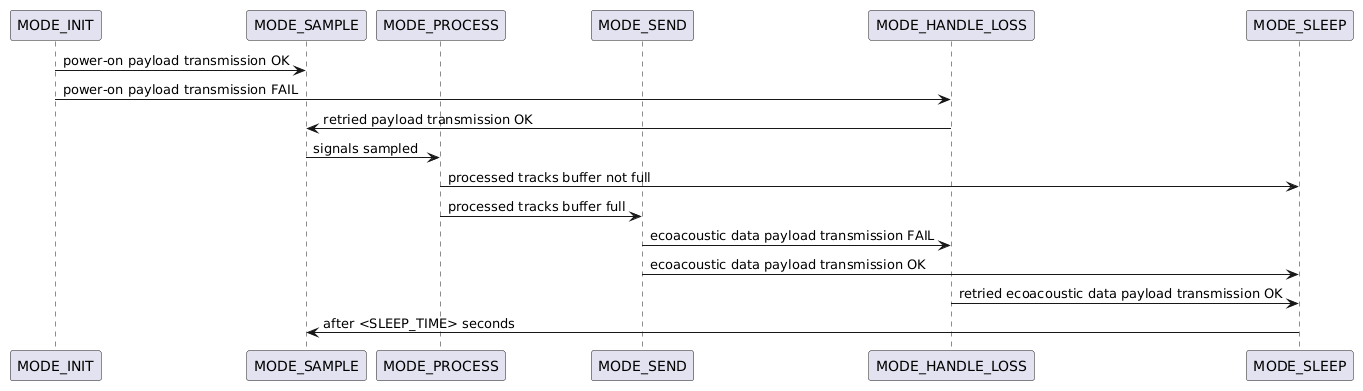
\includegraphics[
            width=\linewidth,
            height=0.72\textheight,
            keepaspectratio
        ]{mode_transitions_diagram.png}
    }{
        \fbox{
            \parbox[c][5cm][c]{0.9\linewidth}{
                \centering
                Mode-transition diagram not found.\\[0.5em]
                Expected file:
                \texttt{mode\_transitions\_white\_background\_sequence.png}
            }
        }
    }

    \caption{Firmware operating-mode transitions.}
    \label{fig:mode-transitions}
\end{figure}

\subsubsection{\modeinit{} Mode}

\begin{requirement}{001}
When the system is powered on, the firmware shall enter \modeinit{}.

In this mode, the firmware shall:

\begin{itemize}
    \item initialize all hardware components required for system operation;
    \item initialize all software components required for system operation;
          and
    \item establish an Internet connection.
\end{itemize}
\end{requirement}

\begin{requirement}{002}
While operating in \modeinit{}, after the required hardware and software
components have been initialized and an Internet connection has been
established, the firmware shall transmit the power-on payload to the cloud.

The payload definitions are provided in
Section~\ref{section:definition}.
\end{requirement}

\begin{requirement}{003}
While operating in \modeinit{}, if transmission of the power-on payload fails,
the firmware shall:

\begin{itemize}
    \item store the transmission failure reason; and
    \item transition to \modehandleloss{}.
\end{itemize}
\end{requirement}

\begin{requirement}{004}
While operating in \modeinit{}, after the power-on payload has been
successfully transmitted to the cloud, the firmware shall transition to
\modesample{}.
\end{requirement}

\subsubsection{\modesample{} Mode}

\begin{requirement}{005}
While operating in \modesample{}, the firmware shall sample the audio signal
and construct an audio track with a duration of
\placeholder{TRACK\_LENGTH} seconds.

The firmware shall use:

\begin{itemize}
    \item I2S to communicate with the audio sensor; and
    \item EasyDMA to retrieve the audio samples.
\end{itemize}

The following sampling parameters shall be used:

\begin{itemize}
    \item \textbf{Number of channels:}
          \placeholder{NUM\_CHANNELS} (TBD);

    \item \textbf{Sample rate:}
          \placeholder{AUDIO\_SAMPLE\_RATE} (TBD);

    \item \textbf{Bandwidth:}
          configurable at compile time through Kconfig; and

    \item \textbf{Sample width:}
          24 bits.
\end{itemize}
\end{requirement}

\begin{requirement}{006}
The firmware shall detect audio-buffer overrun events.

A buffer overrun occurs when the audio sensor advances beyond the firmware's
ability to retrieve the buffered samples.

If a buffer overrun occurs, the firmware shall:

\begin{itemize}
    \item reset the system;
    \item discard any unsent tracks; and
    \item re-enter \modeinit{} as a consequence of the reset.
\end{itemize}
\end{requirement}

\begin{requirement}{007}
If audio acquisition fails while the firmware is operating in
\modesample{}, including failures caused by unrecoverable audio-capture
errors, the firmware shall:

\begin{itemize}
    \item reset the system;
    \item discard any unsent tracks; and
    \item re-enter \modeinit{} as a consequence of the reset.
\end{itemize}
\end{requirement}

\begin{requirement}{008}
While operating in \modesample{}, after an audio track has been recorded,
the firmware shall:

\begin{itemize}
    \item perform a one-shot sampling of temperature, humidity, and pressure,
          thereby forming an atmospheric sample set;
    \item acquire a timestamp with a resolution of one second; and
    \item transition to \modeprocess{}.
\end{itemize}
\end{requirement}

\subsubsection{\modeprocess{} Mode}

\begin{requirement}{009}
While operating in \modeprocess{}, the firmware shall process the most
recently recorded audio track according to the audio processing algorithm.

After processing, the firmware shall:

\begin{itemize}
    \item transition to \modesleep{} if the number of buffered tracks waiting
          to be transmitted is less than
          \placeholder{NUM\_RECORDED\_TRACKS\_BEFORE\_SEND}; or

    \item transition to \modesend{} otherwise.
\end{itemize}
\end{requirement}

\subsubsection{\modesleep{} Mode}

\begin{requirement}{010}
While operating in \modesleep{}, the firmware shall enter an energy-saving
state for a period of \placeholder{SLEEP\_TIME} seconds.

After this period, the firmware shall transition to \modesample{}.

The start time of the next recording shall be determined according to the
\placeholder{SLEEP\_TIME} value configured for this mode.
\end{requirement}

\subsubsection{\modesend{} Mode}

\begin{requirement}{011}
While operating in \modesend{}, the firmware shall transmit the ecoacoustic
data payload to the cloud using HTTP over LTE-M.

The choice between the HTTP \texttt{PUT} and \texttt{POST} methods is
intentionally left unspecified and shall be determined when further
information about the cloud platform becomes available.
\end{requirement}

\begin{requirement}{012}
While operating in \modesend{}, if transmission of the ecoacoustic data
payload fails, the firmware shall:

\begin{itemize}
    \item store the transmission failure reason; and
    \item transition to \modehandleloss{}.
\end{itemize}
\end{requirement}

\begin{requirement}{013}
While operating in \modesend{}, after the ecoacoustic data payload has been
successfully transmitted to the cloud, the firmware shall transition to
\modesleep{}.
\end{requirement}

\subsubsection{\modehandleloss{} Mode}

\begin{requirement}{014}
While operating in \modehandleloss{}, the firmware shall execute one of two
recovery procedures depending on the Internet connection state.

\paragraph{\retrysend}

If the system is connected to the Internet, the firmware shall retry the
transmission of the payload that caused the transition to
\modehandleloss{}.

The retries shall:

\begin{itemize}
    \item use exponential backoff; and
    \item be performed up to
          \placeholder{NUM\_TIMES\_RETRY\_SEND} times.
\end{itemize}

The following outcomes shall apply:

\begin{itemize}
    \item If a transmission attempt succeeds, the firmware shall transition
          to the mode associated with the successfully transmitted payload.

    \item If the system loses its Internet connection during the transmission
          attempts, the firmware shall proceed to \retryconn{}.

    \item The number of failed transmission and connection attempts shall not
          accumulate across \retrysend{} and \retryconn{}.

    \item If all transmission attempts fail, the firmware shall reset the
          system, discard unsent tracks, and re-enter \modeinit{} as a
          consequence of the reset.
\end{itemize}

\paragraph{\retryconn}

If the system is not connected to the Internet, the firmware shall attempt to
re-establish the Internet connection.

The connection attempts shall:

\begin{itemize}
    \item use exponential backoff; and
    \item be performed up to
          \placeholder{NUM\_TIMES\_TRY\_RECONNECT} times.
\end{itemize}

The following outcomes shall apply:

\begin{itemize}
    \item If a connection attempt succeeds, the firmware shall proceed to
          \retrysend{}.

    \item The number of failed transmission and connection attempts shall not
          accumulate across \retrysend{} and \retryconn{}.

    \item If all connection attempts fail, the firmware shall reset the
          system, discard unsent tracks, and re-enter \modeinit{} as a
          consequence of the reset.
\end{itemize}
\end{requirement}

\begin{requirement}{015}
While operating in \modehandleloss{}, if the time spent in this mode exceeds
\placeholder{MAX\_TIME\_SPENT\_HANDLE\_LOSS} seconds, the firmware shall:

\begin{itemize}
    \item reset the system;
    \item discard any unsent tracks; and
    \item re-enter \modeinit{} as a consequence of the reset.
\end{itemize}

This requirement prevents the interval between consecutive audio recordings
from becoming excessively long.
\end{requirement}

\subsection{Usability Requirements}

\begin{requirement}{016}
In all operating modes, the firmware shall log information relevant to:

\begin{itemize}
    \item verifying correct system operation; and
    \item identifying and diagnosing failures.
\end{itemize}

The logs shall be available for real-time monitoring through the system's USB
interface.
\end{requirement}

\subsection{Design Constraints}

The firmware shall be designed so that relevant LTE-M parameters can be
readily adapted to the regulatory requirements of different geographical
regions.

% =============================================================================
\section{Verification}
% =============================================================================

Each requirement shall be verified through analysis of the logs generated by
the firmware, as specified in Requirement~\#016.

When applicable, verification shall also include analysis of the data
received by the cloud platform.

For requirements that specify different outcomes under different conditions,
each condition and its corresponding outcome shall be independently tested.

\subsection{Firmware Test Image}

The firmware shall provide an option for building a dedicated test image.

This test image shall be used to verify:

\begin{itemize}
    \item that audio tracks are recorded according to Requirement~\#005; and
    \item that the audio processing algorithm specified in Requirement~\#009
          is correctly implemented.
\end{itemize}

The test image shall not operate according to the modes described in
Section~\ref{section:modes}.

Instead, it shall:

\begin{itemize}
    \item initialize only the hardware and software components required for
          the verification procedures; and
    \item provide a command-line interface through the system's USB
          interface.
\end{itemize}

The command-line interface shall support the following commands:

\begin{description}[
    style=nextline,
    leftmargin=0pt,
    labelindent=0pt,
    font=\ttfamily
]

    \item[recordAudioTrack]
    Record an audio track and transmit its samples through the USB logging
    interface.

    \item[processAudioTrack]
    Record an audio track, transmit its samples through the USB logging
    interface, process the track according to the audio processing algorithm,
    and transmit the processing results through the USB logging interface.

\end{description}

% =============================================================================
\appendix
\section{Assumptions and Dependencies}
% =============================================================================

It is assumed that the audio processing algorithm and all associated
implementation details will be specified externally.

Therefore, the detailed specification of the audio processing algorithm is
outside the scope of this document.

\end{document}

